
\chapter{Traslación de objetos}

\lettrine[lines=1]{C}{ecilia decidió} que era momento de ponerse a
escribir:

\begin{figure}[ht]
  \begin{minipage}[]{.4\textwidth}
    \begin{lstlisting}
$fn = 200;

sphere(r=10);
cube([25,10,20]);
cylinder(h=15,r=5);
    \end{lstlisting}%$
  \end{minipage}\hfill
   \begin{minipage}[]{.6\textwidth}
     \centering
     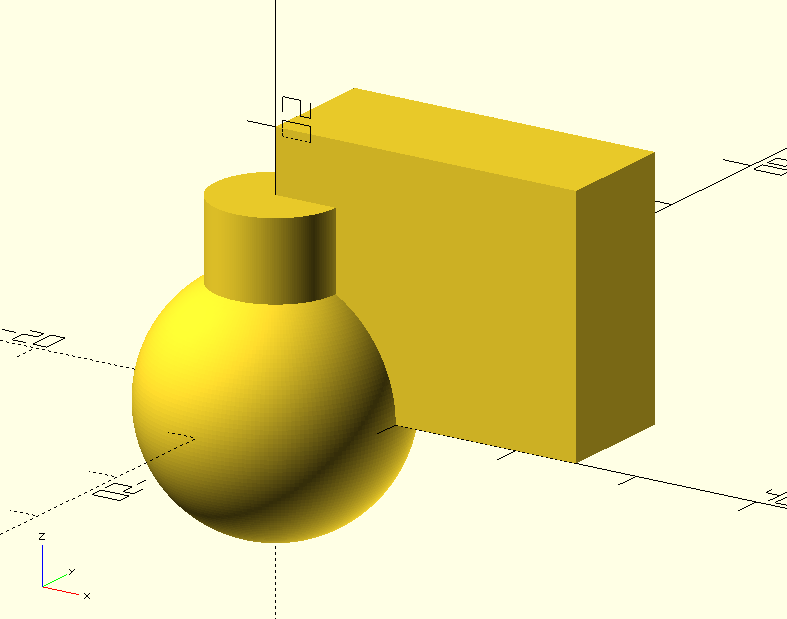
\includegraphics[width=.95\textwidth]{imagenes/esfera-cubo-cilindro-1}
   \end{minipage}
     \caption{Cecilia escribe sus primeros objetos.}
  \label{fig:esfera-cubo-cilindro-1}
\end{figure}



---Lindo ---dijo Antonia displicentemente, y Cecilia sintió que sus
mejillas levantaban temperatura: le molestaba sobremanera la sola
posibilidad de que se burlaran de ella.

---Estoy probando, ¿ok? ---dijo con tono seco, y a\-gre\-gó---:
¿Serías tan amable de indicarme cómo hago para desplazar los
objetos, a fin de que no se solapen o que, en todo caso, lo hagan
donde yo quiera?

 \section{\texttt{center=true}}


 ---Sí, por supuesto ---Antonia pareció no notar el disgusto de
 Cecilia; esa curiosa insensibilidad no era rara en ella, por otro
 la\-do---. En primer lugar, habrás notado que los
 cubos\footnote{Recordamos al lector que un término más ajustado sería
   \emph{ortoedro}, pero en fin. (Nota del Editor)} surgen con uno de
 sus vértices coincidiendo con el origen de coordenadas:

\begin{figure}[ht]
  \begin{minipage}[]{.5\textwidth}
    \begin{lstlisting}[numbers=none]
cube([25,10,20]);
    \end{lstlisting}
  \end{minipage}\hfill
   \begin{minipage}[]{.5\textwidth}
     \centering
     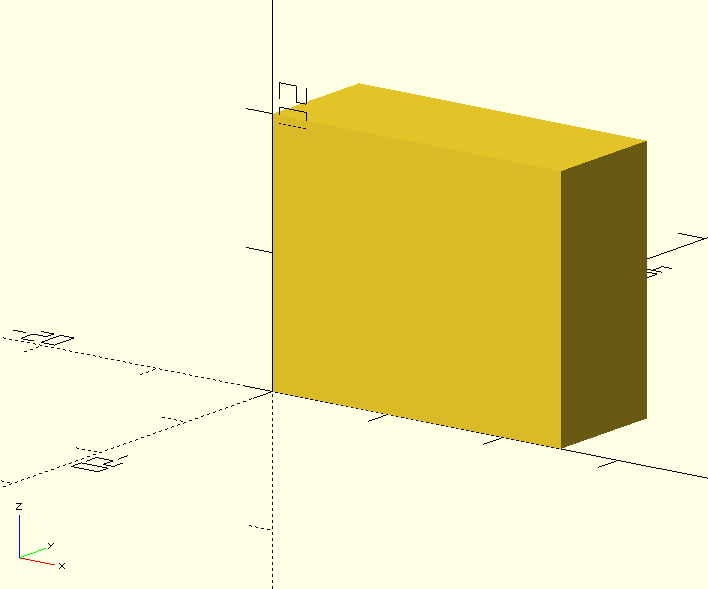
\includegraphics[width=\textwidth]{imagenes/cubo-1}
   \end{minipage}
   \caption{Un \lstinline!cube! es creado con un vértice en el origen
     de coordenadas...}
  \label{fig:cubo-1}
\end{figure}


\guillemotright Si querés que aparezcan centrados en dicho origen
debés agregar la indicación \lstinline!center=true! ---explicó,
mientras escribía el ejemplo de la figura \ref{fig:cubo-2}.

\begin{figure}[ht]
  \begin{minipage}[]{.6\textwidth}
    \begin{lstlisting}[numbers=none]
cube([25,10,20],center=true);
    \end{lstlisting}
  \end{minipage}\hfill
   \begin{minipage}[]{.4\textwidth}
     \centering
     \iftoggle{libro}{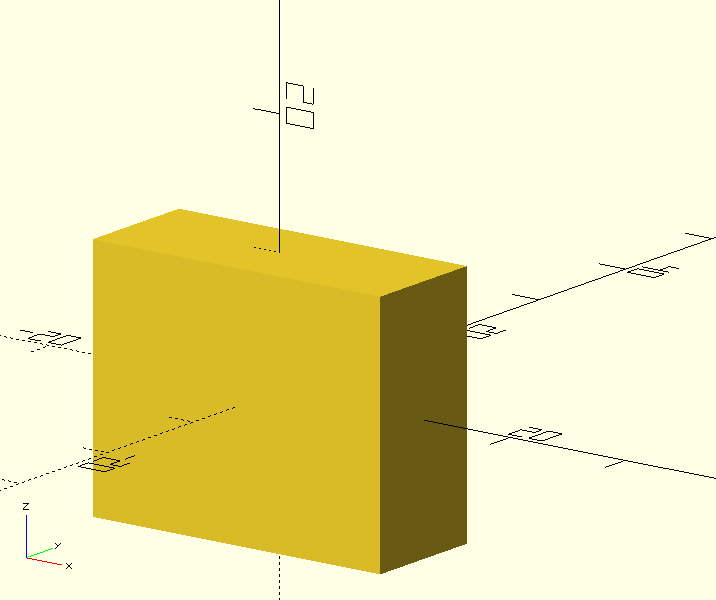
\includegraphics[width=.8\textwidth]{imagenes/cubo-2}}{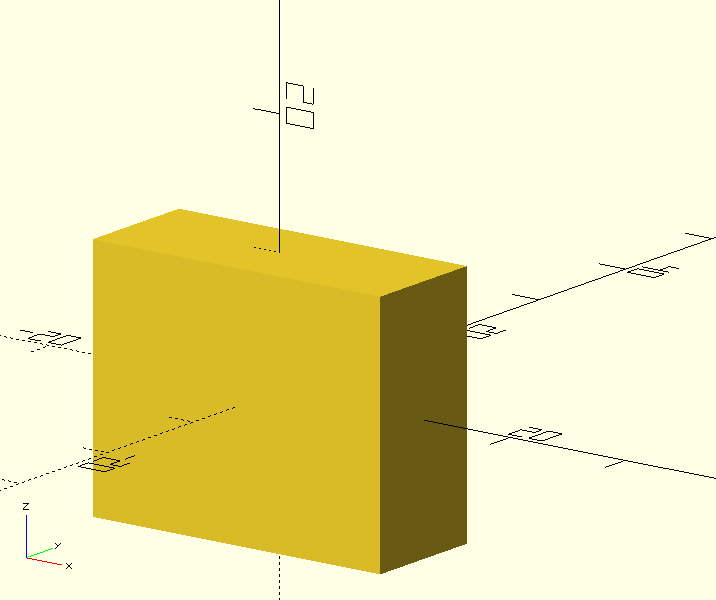
\includegraphics[width=\textwidth]{imagenes/cubo-2}}
     
   \end{minipage}
   \caption{...salvo que reciba la indicación suplementaria
     \lstinline!center=true!.}
  \label{fig:cubo-2}
\end{figure}


\guillemotright Las esferas, por su parte, aparecen centradas en el
origen de coordenadas de por sí. En el caso de los cilindros, en
principio son creados con su eje centrado en el eje \coord{Z} y su
base apoyada en el plano \coord{XY} ---dijo, demostrándolo en la
figura \ref{fig:cilindro-1}.

\begin{figure}[ht]
  \begin{minipage}[]{.5\textwidth}
    \begin{lstlisting}
$fn = 200;
      
cylinder(h=15,r=5);
    \end{lstlisting}%$
  \end{minipage}\hfill
   \begin{minipage}[]{.5\textwidth}
     \centering
     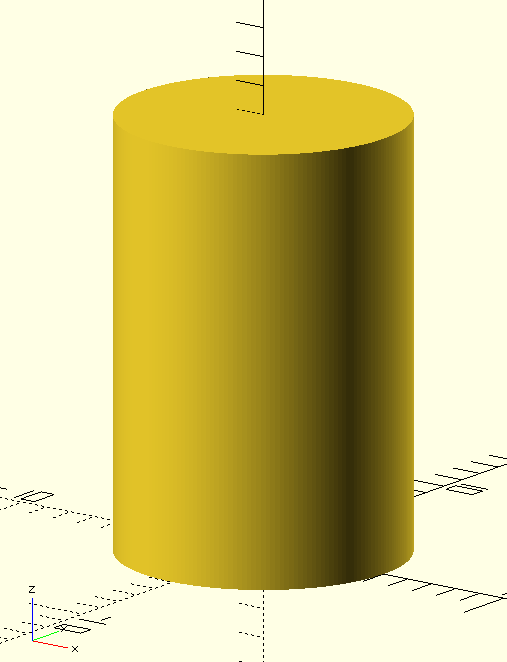
\includegraphics[width=.6\textwidth]{imagenes/cilindro-1}
   \end{minipage}
   \caption{Un \lstinline!cylinder! es creado apoyado sobre el plano
     \coord{XY}...}
  \label{fig:cilindro-1}
\end{figure}

\guillemotright Por otra parte, el añadido \lstinline!center=true!
provoca que \emph{todo} el cuerpo del cilindro resulte centrado con
respecto al origen, como podés apreciar en la figura
\ref{fig:cilindro-2}.

\begin{figure}[ht]
  \begin{minipage}[]{.5\textwidth}
    \begin{lstlisting}
$fn = 200;
      
cylinder(h=15, r=5, center=true);
    \end{lstlisting}%$
  \end{minipage}\hfill
   \begin{minipage}[]{.4\textwidth}
     \centering
     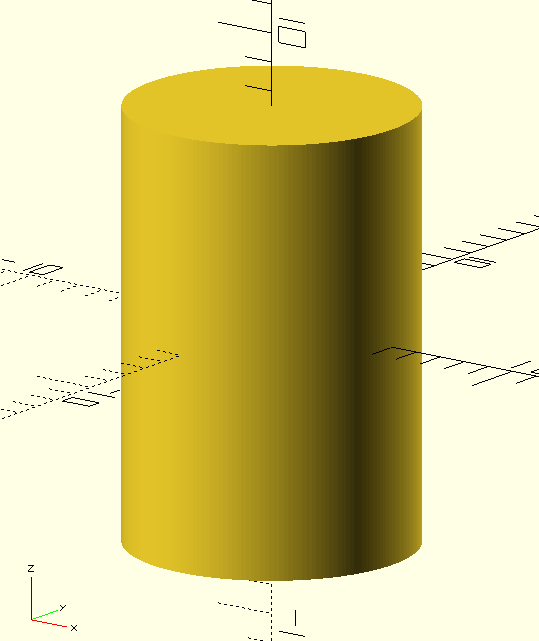
\includegraphics[width=.8\textwidth]{imagenes/cilindro-2}
   \end{minipage}
   \caption{...mas con la indicación \lstinline!center=true! resulta
     centrado en el origen de coordenadas.}
  \label{fig:cilindro-2}
\end{figure}


\section{\texttt{translate}}

\guillemotright Ahora bien, para trasladar un objeto de la manera
más general posible debés precederlo por la indicación
\lstinline!translate! ---anunció Antonia, escribiendo el ejemplo de la
figura \ref{fig:esfera-cubo-cilindro-2}.

\begin{figure}[ht]
  \begin{minipage}[]{.45\textwidth}
    \begin{lstlisting}
$fn = 200;

sphere(r=10);

translate([15,-5,-10])
  cube([25,10,20]);
  
translate([-20,0,-7.5])  
  cylinder(h=15,r=5);
    \end{lstlisting}%$ 
  \end{minipage}\hfill
   \begin{minipage}[]{.55\textwidth}
     \centering
     \iftoggle{libro}{%
       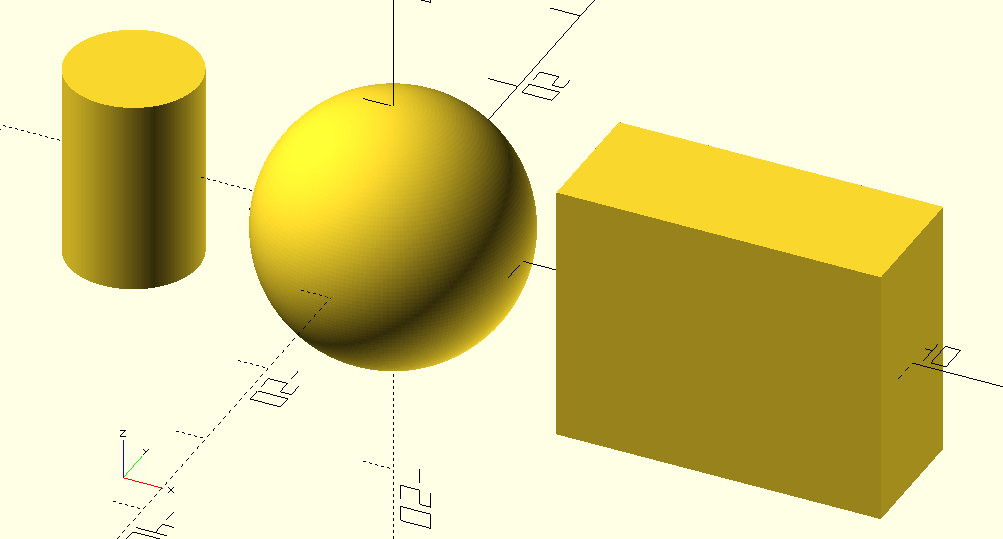
\includegraphics[width=.8\textwidth]{imagenes/esfera-cubo-cilindro-2}}{%
       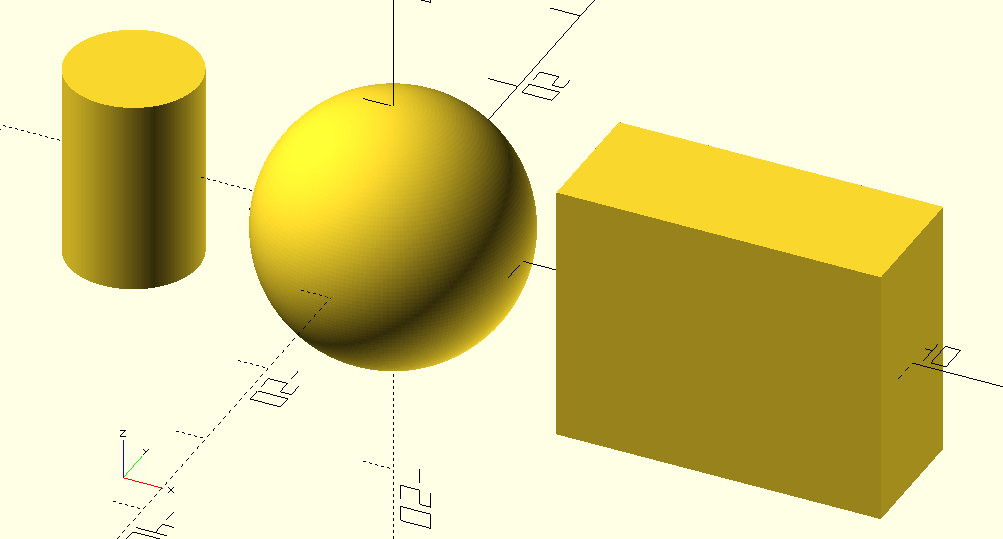
\includegraphics[width=.95\textwidth]{imagenes/esfera-cubo-cilindro-2}}       
   \end{minipage}
   \caption{La transformación \lstinline!translate! permite colocar un
     objeto donde al escritor le plazca.}
   \label{fig:esfera-cubo-cilindro-2}
\end{figure}


Cecilia se acercó involuntariamente a la pantalla, entrecerrando
ligeramente los ojos mientras analizaba lo escrito por Antonia. La
instrucción \lstinline!translate! parecía bastante elocuente:
trasladaba el objeto al cual se aplicaba a continuación una cierta
distancia en \coord{X}, \coord{Y} y \coord{Z}. En el caso particular
del cubo reciente lo movía 15mm en \coord{X}, por ejemplo. Le pareció
simpático el empleo de números negativos: mover el cubo -10mm en
\coord{Z} equivalía a hacerlo descender.

---Fijate que la línea \lstinline!translate! no termina con un punto y
coma ---Antonia parecía sentir a veces la necesidad de interrumpir los
pensamientos de Cecilia---; eso se debe a que no es una instrucción en
sí misma, sino que es una suerte de transformación que se aplica al
objeto inmediato siguiente.

---Suena lógico ---dijo ésta tras considerarlo unos intantes, y
preguntó:

---¿Son necesarios los dos espacios que preceden a \lstinline!cube!  y
\lstinline!cylinder!  en el texto?

---No ---respondió Antonia---; son otra mera comodidad visual. Podés
omitirlos si querés. De hecho, podés escribir
\begin{lstlisting}[numbers=none]
translate([15,-5,-10])cube([25,10,20]);
\end{lstlisting}
\noindent en una misma línea y funciona igual. Con el tiempo, y a
medida que escribas, vas a encontrar la mejor disposición visual para
tus textos; lo importante es que resulten visualmente claros. La
claridad en este género literario, no sólo en cuanto al contenido
semántico sino en el aspecto meramente visible, es fundamental: vas a
descubrir que tus propios textos pueden resultarte extraños tras unos
días de no frecuentarlos. En esos momentos agradecerás haberlos
escrito de la manera más clara posible.

Cecilia sintió que ahora podía escribir algo bastante más
bonito. Después de un buen rato consiguió enhebrar unas cuantas
esferas:

    \begin{lstlisting}
$fn = 200;
      
sphere(r=16);
translate([0,0,24])
  sphere(r=8);
translate([0,0,36])
  sphere(r=4);
translate([0,0,42])
  sphere(r=2);
translate([0,0,45])
  sphere(r=1);
translate([0,0,46.5])
  sphere(r=.5);
translate([0,0,47.25])
  sphere(r=.25);    
    \end{lstlisting}%$


\begin{figure}[ht]
     \centering
     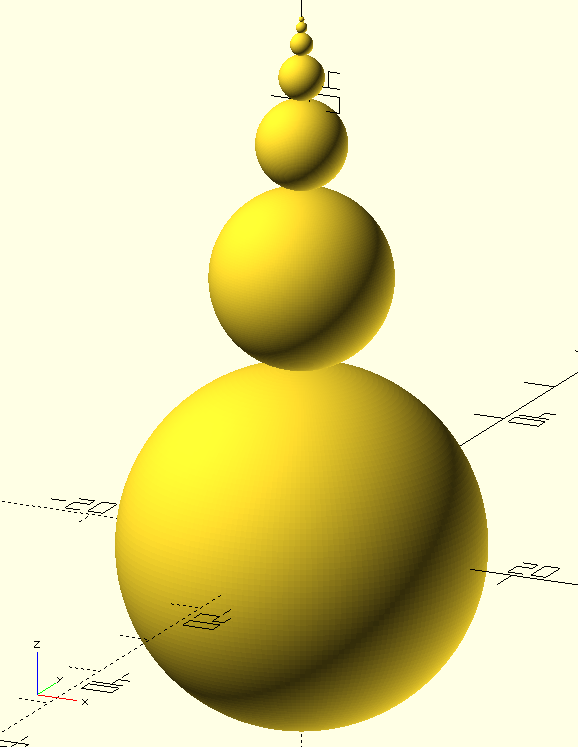
\includegraphics[width=.6\textwidth]{imagenes/esferas}
   \caption{Cecilia se anima y apila una serie de esferas.}
   \label{fig:esferas}
\end{figure}

---No está mal... ---aprobó Antonia, admirando con una amplia sonrisa
la figura \ref{fig:esferas}.

Cecilia estuvo de acuerdo, y siguió jugando:

    \begin{lstlisting}
$fn = 200;
      
sphere(r=16);
translate([0,0,24])
  sphere(r=8);
translate([0,0,36])
  sphere(r=4);
translate([0,0,42])
  sphere(r=2);
translate([0,0,45])
  sphere(r=1);
translate([0,0,46.5])
  sphere(r=.5);
translate([0,0,47.25])
  sphere(r=.25);

translate([60,0,0])
  cube([32,32,32],center=true);
translate([60,0,24])
  cube([16,16,16],center=true);
translate([60,0,36])
  cube([8,8,8],center=true);
translate([60,0,42])
  cube([4,4,4],center=true);
translate([60,0,45])
  cube([2,2,2],center=true);
translate([60,0,46.5])
  cube([1,1,1],center=true);
translate([60,0,47.25])
  cube([0.5,0.5,0.5],center=true);
    \end{lstlisting}%$

    
\begin{figure}[ht]
  \centering
  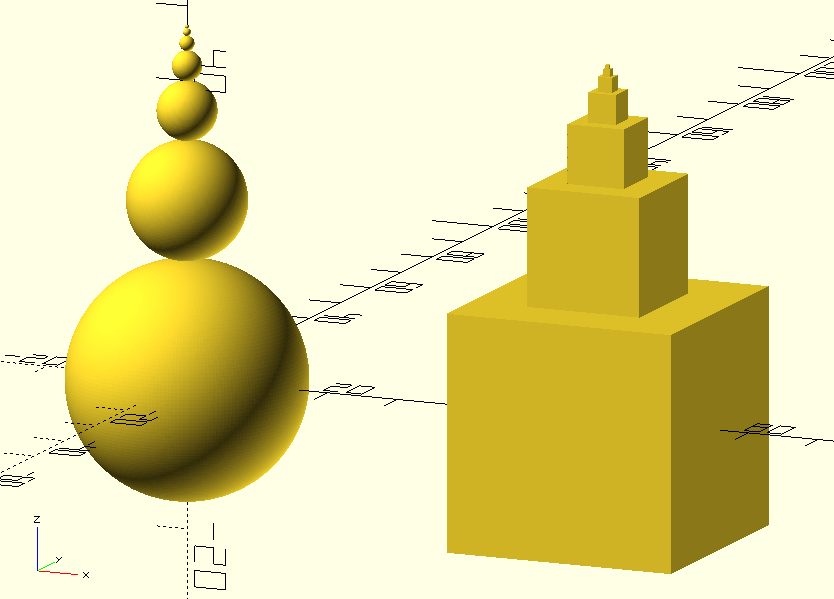
\includegraphics[width=.9\textwidth]{imagenes/esferas-cubos}
  \caption{Esferas y cubos apilados por Cecilia.}
  \label{fig:esferas-cubos}
\end{figure}


---¡Extraordinario! ---exclamó Antonia, y en sus ojos bailaba un
fulgor especial mientras contemplaba alternativamente el texto de
Cecilia y la figura \ref{fig:esferas-cubos}---. Este texto me encanta,
porque nos va a permitir reflexionar un poco sobre el problema
particular que atrapó tu atención.

---¿Qué problema particular? ---preguntó Cecilia con cándida
sinceridad---. Sólo quise poner en práctica los poquitos elementos que
vimos hasta ahora.

---En principio, es posible que así haya sido ---replicó Antonia
fingiendo paciencia---. Pero podrías haberlo hecho de mil modos
distintos. Pensemos juntas \emph{por qué} elegiste éste y no
otro. ¡Ojo!  ---se atajó---; no estoy pensando en hacerte
psicoanálisis a la violeta; si querés, digamos que vamos a analizar el
texto a ver qué nos cuenta.

Cecilia, incluso acostumbrada a las excentricidades de Antonia, no
pudo evitar cierto recelo.

 

%%% Local Variables:
%%% mode: latex
%%% TeX-master: "../libro"
%%% End:
